\chapter{如何說得有意義}

無論我們是背稿、照稿讀、只看幾條筆記，還是完全不看任何提示，這場講座都先堅持一個更前面的要點：一場準備充分、又帶著熱情講出的演講，依然可以打動聽眾。這個開頭並不是隨意的鼓勵，而是在先清除一個錯誤問題，好把我們重新導向真正的核心。既然文字早已寫在紙上，現場講述究竟額外帶來了什麼？答案一步步展開。演講之所以重要，是因為它替資訊加上了一層人的維度；而這一層，必須透過兩個我們確實能掌控的變數來組織：聲音與身體。

\section{既然如此，為什麼不直接把稿子寄出去？}

講座一開始，便把整個主題轉化成一個尖銳而實際的問題。既然話都已經寫好了，為什麼還要站到眾人面前把它說出來？為什麼不乾脆把稿子寄給所有本來會來聽的人？

這是一個正確的開場問題，因為它拒絕讓「說話」躲在儀式感背後。若現場演講並未帶來任何本質性的東西，那麼現場演講就只是一種昂貴而多餘的重複。因此，講者把壓力直接施加在媒介本身之上。口說這件事，到底做了哪些書面頁面做不到的事？

最初的對比可以示意地寫成：
\begin{equation}
\text{單獨的印刷文字} \neq \text{帶有人性層次的現場演講}.
\end{equation}

\subsection{Question \& Answer}

\paragraph{Question.} 如果文字都已經寫好了，為什麼還要演講，而不是直接把文本寄出去？

\paragraph{Answer.} 因為演講不只是把句子送出去的管道。在現場言說中，聽眾接收到的不僅是資訊，還有講者的在場。聲音與身體能夠改變注意力、強調、信任、迫切感與情感上的接受方式，而這些都不是一張紙本身所能完成的。

開場投影片以一種刻意剝除細節的形式記下了這個傳輸問題。一個中心，面向許多聽者：
\begin{equation}
\text{講者／訊息} \longrightarrow \text{聽眾成員}.
\end{equation}

\begin{figure}[h]
\centering

\includegraphics[width=0.58\textwidth]{how_to_speak_with_meaning_figure_02.png}
\end{figure}

\begin{figure}[h]
\centering
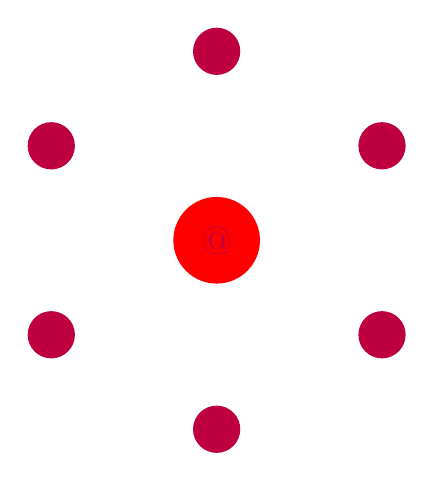
\begin{tikzpicture}[scale=1.0]
\fill[red] (0,0) circle (0.55);
\node[color=purple] at (0,0) {\Large @};

\fill[purple] (0,2.4) circle (0.30);
\fill[purple] (2.1,1.2) circle (0.30);
\fill[purple] (2.1,-1.2) circle (0.30);
\fill[purple] (0,-2.4) circle (0.30);
\fill[purple] (-2.1,-1.2) circle (0.30);
\fill[purple] (-2.1,1.2) circle (0.30);
\end{tikzpicture}
\end{figure}

投影片本身是抽象的。它還沒有回答問題。它只是先固定了問題的幾何結構：如果訊息可以從中央向外分送，那麼表演性的必要性究竟在哪裡？講座接下來的動作，便不是靠比喻，而是靠效果來回答。

\section{人性把資訊轉化為啟發}

講者說，演講的確能提供超出印刷文字之外的東西，但這份 ``額外之物'' 並不會自動發生。它需要被思考、被投入、被培養，也需要被掙得。這一點很重要。人性的那一層，不會只因為有人站上台就自動成立。它只有在改變了聽者內部發生的事情時，才真正有效。

那種改變看起來像什麼？講座用聽眾心中想像出來的聲音作答：
\begin{itemize}
\item ``我信任這個人。''
\item ``每一句話聽起來都很有意思。''
\item ``我從你的聲音裡聽見，也從你的表情裡看見了。''
\item ``那個詞這樣一強調，再配上那個手勢，我懂了。''
\item ``我感覺得到那件事對你有多痛。''
\item ``那種熱情會傳染。''
\item ``那雙眼裡有一種決心。''
\item ``我想站到你這一隊。''
\end{itemize}

這一串安排得很精巧。信任、興趣、強調、同理、興奮、信念與行動，並不是各自獨立的裝飾，而是資訊如何在另一個心靈中變得活躍起來的一連串方式。

\subsection{Question \& Answer}

\paragraph{Question.} 現場演講相較於稿子，多出來的那個 ``額外之物'' 到底是什麼？

\paragraph{Answer.} 它就是我們的人性，但這裡的人性是以操作性的方式被理解的：那層可聽見、也可看見的部分，改變了聽眾接收同一份資訊的方式。當講者的在場，把意義轉化為某種可被感受、被信任、並被付諸行動的東西時，演講便不再只是文字。

講座把整條鏈壓縮成一個主導性的詞：
\begin{equation}
\text{人性} + \text{資訊} \Longrightarrow \text{啟發}.
\end{equation}

\begin{definition}
在這場講座裡，\emph{啟發} 指的是這樣一種力量：它會告訴心靈，拿一個新想法來做什麼，而不是讓它被歸檔之後就此遺忘。
\end{definition}

這便給了我們一個清楚的對比：
\begin{align}
\text{普通的想法} &\Longrightarrow \text{被歸檔收起}, \\
\text{啟發} &\Longrightarrow \text{喚醒注意力}.
\end{align}

這個轉折，才是整場講座真正的鉸鏈。我們最初從一個關於說話與寫作的社會性問題出發，而現在則被帶到一個功能性的定義上。一旦啟發是根據它所造成的效果來界定的，講者終於可以追問：在講者身上，究竟有哪些變數能夠控制它？

\section{兩件最重要的事}

到了這裡，講座從效果轉向方法。如果目標是啟發，那麼在準備演講時，我們主要應該處理哪些事情？答案驚人地節制：只有兩件大事要考慮。我們正在如何使用自己的聲音？我們又正在如何使用自己的身體？

這種拆分非常重要，因為它阻止整場討論溶解成泛泛而談的建議。講座並沒有告訴我們要 ``有魅力'' 或 ``有熱情''，而是把整個場域縮減成兩個可以被控制的變數，然後逐一加以考察。

\subsection{Question \& Answer}

\paragraph{Question.} 準備一場演講時，我們真正應該優化的兩件事是什麼？

\paragraph{Answer.} 我們應該優化兩件事：聲音，因為它決定意義如何被聽見；身體，因為它決定自信、強調與沉著如何被看見。

這個結構性分裂，可以寫成
\begin{equation}
\text{演講準備} \Longrightarrow \text{聲音} + \text{身體}.
\end{equation}

對應的投影片並不是把這件事當作一條明白標示的定理，而是用一種分叉形式呈現：上方是一個大問題，中間是一個決策點，下方則是相互對照的兩條路徑。

\begin{figure}[h]
\centering

\includegraphics[width=0.68\textwidth]{how_to_speak_with_meaning_figure_03.png}
\end{figure}

\begin{figure}[h]
\centering
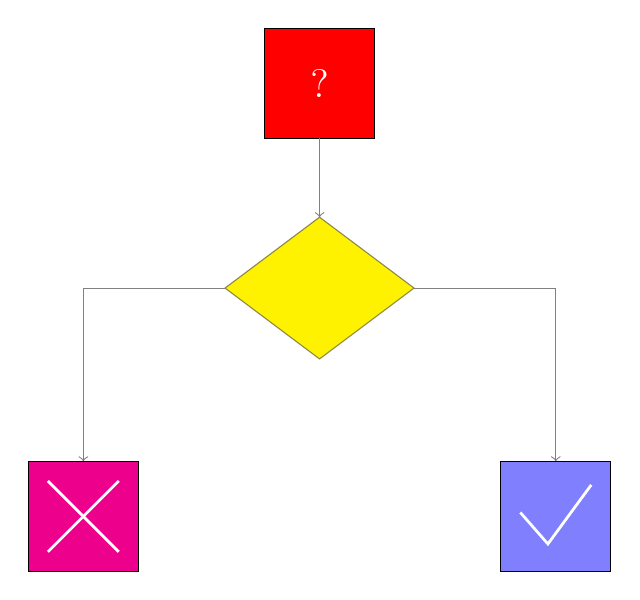
\begin{tikzpicture}[scale=1.0]
\draw[fill=red] (-0.7,2.4) rectangle (0.7,3.8);
\node[color=white] at (0,3.1) {\Large ?};

\draw[->, gray] (0,2.4) -- (0,1.4);

\draw[fill=yellow, draw=yellow!50!black] (0,1.4) -- (-1.2,0.5) -- (0,-0.4) -- (1.2,0.5) -- cycle;

\draw[gray] (-1.2,0.5) -- (-3.0,0.5) -- (-3.0,-1.0);
\draw[gray] (1.2,0.5) -- (3.0,0.5) -- (3.0,-1.0);
\draw[->, gray] (-3.0,-1.0) -- (-3.0,-1.7);
\draw[->, gray] (3.0,-1.0) -- (3.0,-1.7);

\draw[fill=magenta] (-3.7,-3.1) rectangle (-2.3,-1.7);
\draw[white, line width=1pt] (-3.45,-2.85) -- (-2.55,-1.95);
\draw[white, line width=1pt] (-3.45,-1.95) -- (-2.55,-2.85);

\draw[fill=blue!50] (2.3,-3.1) rectangle (3.7,-1.7);
\draw[white, line width=1pt] (2.55,-2.35) -- (2.9,-2.75) -- (3.45,-2.0);
\end{tikzpicture}
\end{figure}

這張圖比逐字稿更抽象。逐字稿則透過命名兩條分支，解決了這個結構。這樣的順序值得保留在頁面上。我們先看見分裂的形式，然後才被告知，究竟是什麼填滿了它。

\section{聲音：依意義而變化}

講者進入第一條分支，也就是聲音，靠的不是規則，而是範例。我們被帶去看 George Monbiot 的開場一分鐘，先感受效果，然後才被告知這效果是如何被製造出來的。這一點在教學上很重要。我們先聽見現象，之後才為它命名。

Monbiot 那段軼事的細節，並不是這裡的重點，而且逐字稿在那一段也有些許失真。真正重要的是圍繞它的穩定教訓。他的聲音替每一個字加上了意義。聽眾之所以被拉進他的世界，不只是因為文字本身寫得好，而是因為他的講法在這些字句之間做出了區別。有些片語被展開，有些片語被收緊，有些想法被允許真正落地。我們聽見的，不只是順序，而是結構。

\subsection{Question \& Answer}

\paragraph{Question.} 講者如何讓字句不只是正確，而是真正活起來？

\paragraph{Answer.} 靠的是說話方式中的變化，而且這種變化必須回應意義。好的聲音變化不是裝飾性的，而是語義性的。它告訴聽眾，哪裡有重量。

因此，主導規則便是
\begin{equation}
\text{言說中的變化} \Longrightarrow \text{使意義變得可聽見}.
\end{equation}

接著，講座又用一個反例把這個要點說得更尖銳。並不是每一場演講都能帶來那層額外的人性。有些演講會把自己壓平。每一句話都用同樣的輪廓、同樣微小的起伏、同樣的速度、同樣的壓力講出來。於是聽眾收到的便是一個錯誤訊號：
\begin{equation}
\text{每一句話都聽起來一樣} \Longrightarrow \text{沒有任何一部分顯得比其他部分更重要}.
\end{equation}

這也就是為什麼講座會把這種說話比作一種壞意義上的催眠：它會把聽眾慢慢哄睡。問題不只是無聊，而是結構性的。單一而平坦的聲音，剝奪了論證本應有的層級。

\section{在稿子上做記號，好讓聲音能動起來}

一旦這個診斷完成，講座就轉入程序。如果演講是有稿的，講者告訴我們，不應被動地等待聲音變化自己出現。我們應當把這些變化先建入頁面之中。換言之，我們是在稿子之上，再寫出一套關於講法的記號。

這是整場講座最有力的時刻之一，因為它用一個可執行的演算法，取代了模糊的建議。我們先從局部開始，一句一句處理，再從局部升到整體，一段一段處理。

\subsection{Question \& Answer}

\paragraph{Question.} 如果演講有稿，該如何在稿子上做記號，讓聲音依意義而變化，而不會滑進單調？

\paragraph{Answer.} 我們先在每一句裡畫出最重要的兩三個字。接著，在每一段中找出那個真正最關鍵的詞，替它畫雙底線。然後再針對局部特殊效果加上專屬標記：俏皮之處、問句、笑點，以及整場最主要的 aha 時刻。

講座中的記號系統，首先建立在句子層次與段落層次的區分之上：
\begin{align}
\text{句子} &\mapsto \underline{\text{重要詞語}}, \\
\text{段落} &\mapsto \underline{\underline{\text{一個主導詞}}}.
\end{align}

那張投影片正好精確地記下了這個結構：像文字一樣的區塊，裡頭有些位置被特地標示出來，要求強調。

\begin{figure}[h]
\centering

\includegraphics[width=0.63\textwidth]{how_to_speak_with_meaning_figure_04.png}
\end{figure}

\begin{figure}[h]
\centering
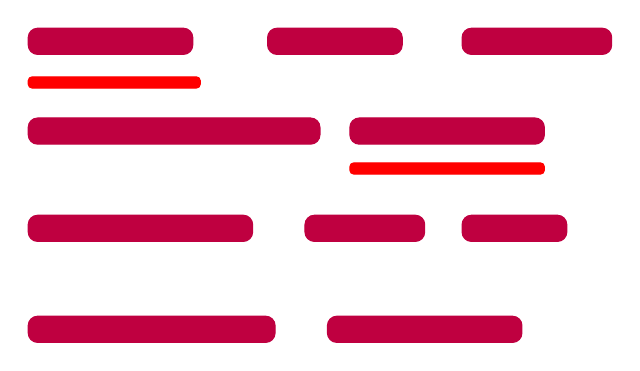
\begin{tikzpicture}[scale=0.95]
\draw[fill=purple, draw=purple, rounded corners=0.12cm] (-3.1,2.4) rectangle (-0.9,2.75);
\draw[fill=purple, draw=purple, rounded corners=0.12cm] (0.1,2.4) rectangle (1.9,2.75);
\draw[fill=purple, draw=purple, rounded corners=0.12cm] (2.7,2.4) rectangle (4.7,2.75);

\draw[fill=red, draw=red, rounded corners=0.05cm] (-3.1,1.95) rectangle (-0.8,2.1);

\draw[fill=purple, draw=purple, rounded corners=0.12cm] (-3.1,1.2) rectangle (0.8,1.55);
\draw[fill=purple, draw=purple, rounded corners=0.12cm] (1.2,1.2) rectangle (3.8,1.55);

\draw[fill=red, draw=red, rounded corners=0.05cm] (1.2,0.8) rectangle (3.8,0.95);

\draw[fill=purple, draw=purple, rounded corners=0.12cm] (-3.1,-0.1) rectangle (-0.1,0.25);
\draw[fill=purple, draw=purple, rounded corners=0.12cm] (0.6,-0.1) rectangle (2.2,0.25);
\draw[fill=purple, draw=purple, rounded corners=0.12cm] (2.7,-0.1) rectangle (4.1,0.25);

\draw[fill=purple, draw=purple, rounded corners=0.12cm] (-3.1,-1.45) rectangle (0.2,-1.1);
\draw[fill=purple, draw=purple, rounded corners=0.12cm] (0.9,-1.45) rectangle (3.5,-1.1);
\end{tikzpicture}
\end{figure}

接著，講座又補上一組第二層的記號：
\begin{align}
\text{問號} &\mapsto \text{提示強調}, \\
\text{俏皮段落} &\mapsto \text{波浪底線}, \\
\text{aha 時刻} &\mapsto \text{前方一個黑色圓點}, \\
\text{笑話或有趣故事} &\mapsto \text{上方的粉紅點}.
\end{align}

這些記號不是裝飾，而是指令。它們是在告訴聲音該怎麼做：
\begin{equation}
\text{稿上記號} \Longrightarrow \text{相應的聲音變化}.
\end{equation}

\paragraph{Worked procedure.} 講座的方法可以寫成一條從稿子走向講述的受控流程。
\begin{enumerate}
\item 一句一句地讀稿，替承擔局部重心的少數詞語畫線。
\item 往上一個層次移動，在每一段裡挑出那個主宰整段運動的單一詞語，替它畫雙線。
\item 對問句、俏皮片段、笑點與主要 aha 時刻，各自加上視覺標記。
\item 再讀一遍，此時讓停頓、速度、輕重與強調依照記號作出回應。
\item 再讀一次，這一回則讓每一部分所帶的情緒狀態進入聲音。
\end{enumerate}

最後這一步，防止整套程序淪為機械操作。講座明白要求我們記起演講各部分所附著的情緒：哪些段落會引發熱情、憤怒、笑聲或困惑。只有到這時，這些記號才不只是排版符號。檢查的方式也很實際：找一位朋友試聽，或者把自己錄下來，然後閉上眼睛回放。

\section{身體：站姿、移動與靜止}

只有在聲音被賦予方法之後，講座才轉向身體。而它再次從一種失效模式開始。有些講者上台時，彷彿身體只是用來搬運頭顱的容器。一旦站到台上，整個身體便變得遲疑：雙手垂在身側、重心來回挪動、動作存在卻沒有意圖。

講者的第一個處方異常簡單。站直。雙腳平均承重。雙腳相距數英寸。重點不在舞台上的宏偉氣勢，而在於先建立一個穩定的底座，讓身體其餘部分變得可讀。

\subsection{Question \& Answer}

\paragraph{Question.} 講者應該站著不動，還是在台上走動？

\paragraph{Answer.} 兩者都可以。但靜止必須是可用的，而移動必須有目的。聽眾應該看見節奏與控制，而不是內在不安向外滲漏的痕跡。

可見的投影片，以符號形式給出了關鍵關係：
\begin{equation}
\text{左腳的重量} = \text{右腳的重量}.
\end{equation}

\begin{figure}[h]
\centering

\includegraphics[width=0.56\textwidth]{how_to_speak_with_meaning_figure_05.png}
\end{figure}

這條等式是審慎重建的結果。畫面裡能清楚看見等號；左右兩側所詮釋的變數，則由逐字稿補足。但這個重建是忠於講座意思的。身體上的平衡，是沉著力量的第一個條件。

一旦這個底座穩住了，上半身便可以開始活動。手與手臂可以自然地幫助強調所說的內容。良好的姿態也有幫助。駝背會削弱訊號。接著，講座又把焦點從站姿擴展到節奏：
\begin{equation}
\text{有目的的移動} + \text{靜止的時刻} \Longrightarrow \text{有力的舞台節奏}.
\end{equation}

對應的警告同樣鮮明：
\begin{equation}
\text{不停踱步或搖晃} \Longrightarrow \text{讓觀眾看見不適}.
\end{equation}

\paragraph{Practical rule.} 關於身體這一側，講座的演算法簡短而具體。
\begin{enumerate}
\item 先建立穩定的底座。
\item 讓手勢出自內容，而不是出自焦慮。
\item 當移動能幫助思考或強調時，就移動。
\item 當一個重要觀點需要落地時，就停下來。
\item 去除反覆的搖晃，因為它所宣告的更多是緊張，而不是意義。
\end{enumerate}

講座裡那句 ``calm power'' 在這裡很貼切。我們不是要把身體凍住，而是要讓它變得可讀。

\section{沒有單一風格，只有舒服而自信的在場}

到了這裡，講座做出了一個必要的修正。在給出若干具體經驗法則之後，它拒絕把這些法則變成一種統一的好演講範本。有些講者坐著演講。有些講者以極大的能量移動。有些則幾乎全程靜止。講者之所以提到 Dame Stephanie Shirley、Oliver Sacks 與 Clifford Stoll，正是為了打破那種模仿的衝動。

這並不是對先前建議的退縮，而是對它們的完成。講座所給出的規則，不是要製造一致性，而是要移除那些本可避免的干擾。當這些干擾被移除之後，不同的舞台風格便能各自綻放，而不會變成分心來源。

因此，最終的標準並不是我們是否長得像某位典範講者，而是我們在台上的存在方式，是否讓自己感到舒服而有自信，並且是否讓觀念能夠乾淨地通過。講座把這個測試保持在非常具體的層次：在一小群觀眾面前排練，或者回看自己的錄影，然後問一個問題：你的身體語言，究竟是在幫助訊息，還是在妨礙訊息？

而這也正是講座悄悄回到最初邏輯的地方。整套傳遞的目的，都是為了讓想法帶著力量抵達。身體不是用來替表演添花的，它本身就是承載意義的裝置之一。

\section{Summary}

整場講座以一種受控的論證方式展開。我們先面對一個挑戰：既然文字早已寫在頁上，為何還要把它大聲說出來？答案是，現場講述能加上一層人的維度，而這一層能把資訊轉化為啟發。一旦這點被理解，講座便把準備工作縮減成兩個我們確實可以處理的變數：聲音與身體。

在聲音這一側，核心原則是：變化必須跟隨意義。聲音應該標出層級，而不是把層級壓平。這也就是為什麼講座提供了一套明確的稿件標記方法：替重要詞語畫底線、替主導整段的詞畫雙底線，並為問句、俏皮、幽默與主要 aha 時刻加上局部記號。在身體這一側，講座先從平衡開始，再擴展到手勢、移動與靜止，而且始終堅持：動作必須服務強調，而不是洩露焦慮。

因此，本章最後回到講座本身結束的地方。沒有唯一一種演講風格值得模仿。我們真正想要的，是一副聲音與一具身體，能讓想法帶著清晰、信念，以及無可錯認的人性在場感穿透出去。